\clearpage{\pagestyle{empty}\cleardoublepage}
\chapter{Contesto}
\lhead[\fancyplain{}{\bfseries\thepage}]{\fancyplain{}{\bfseries\rightmark}}
\pagenumbering{arabic}

In questo capitolo ci si immergerà nell'ambito delle tecnologie digitali emergenti che stanno ridefinendo il panorama tecnologico odierno. Esploreremo in profondità le componenti fondamentali di questo ecosistema, concentrandoci su concetti come il \emph{Digital Twin}, il \emph{Digital Thread} e il \emph{Digital Shadow}.

Questo capitolo si concentrerà prevalentemente sul concetto di \emph{Digital Twin}, esaminando le sue definizioni, la sua evoluzione storica e i vantaggi che offre. Esploreremo anche le categorie e le gerarchie sottostanti, analizzando come questo concetto sia utilizzato in diversi ambiti.

Successivamente, parleremo del \emph{Digital Thread}, esplorando le sue applicazioni e vantaggi. Sarà fondamentale comprendere come questo concetto si integra nell'ecosistema più ampio delle tecnologie digitali.

Infine, affronteremo il concetto di \emph{Digital Shadow}. Esamineremo cosa si intende con questo termine, evidenziando sia i benefici che i possibili problemi che potrà presentare in futuro. In particolare, esploreremo le questioni legate all'etica e alla regolamentazione che sorgono in relazione al concetto di \emph{Digital Shadow}, oltre a esaminare il ruolo fondamentale dell'economia dei dati.

Attraverso l'approfondimento delle sottosezioni all'interno di questo capitolo, otterremo una comprensione completa di come queste tecnologie stanno ridefinendo una serie di settori.


\section{Digital Twin}

Il \emph{Digital Twin} si riferisce alla copia virtuale di qualsiasi entità fisica (la traduzione in italiano è ”gemello fisico”), entrambi interconnessi tramite lo scambio di dati in tempo reale~\cite{NASA}.

L'applicazione del \emph{Digital Twin} include il monitoraggio in tempo reale, la progettazione/pianificazione, l'ottimizzazione, la manutenzione, l'accesso remoto, ecc. La sua implementazione è prevista in crescita esponenziale nei prossimi decenni a giudicare dai \emph{Google trends} (figura \ref{fig:trends}).

\begin{figure}[h]
\begin{center}                      
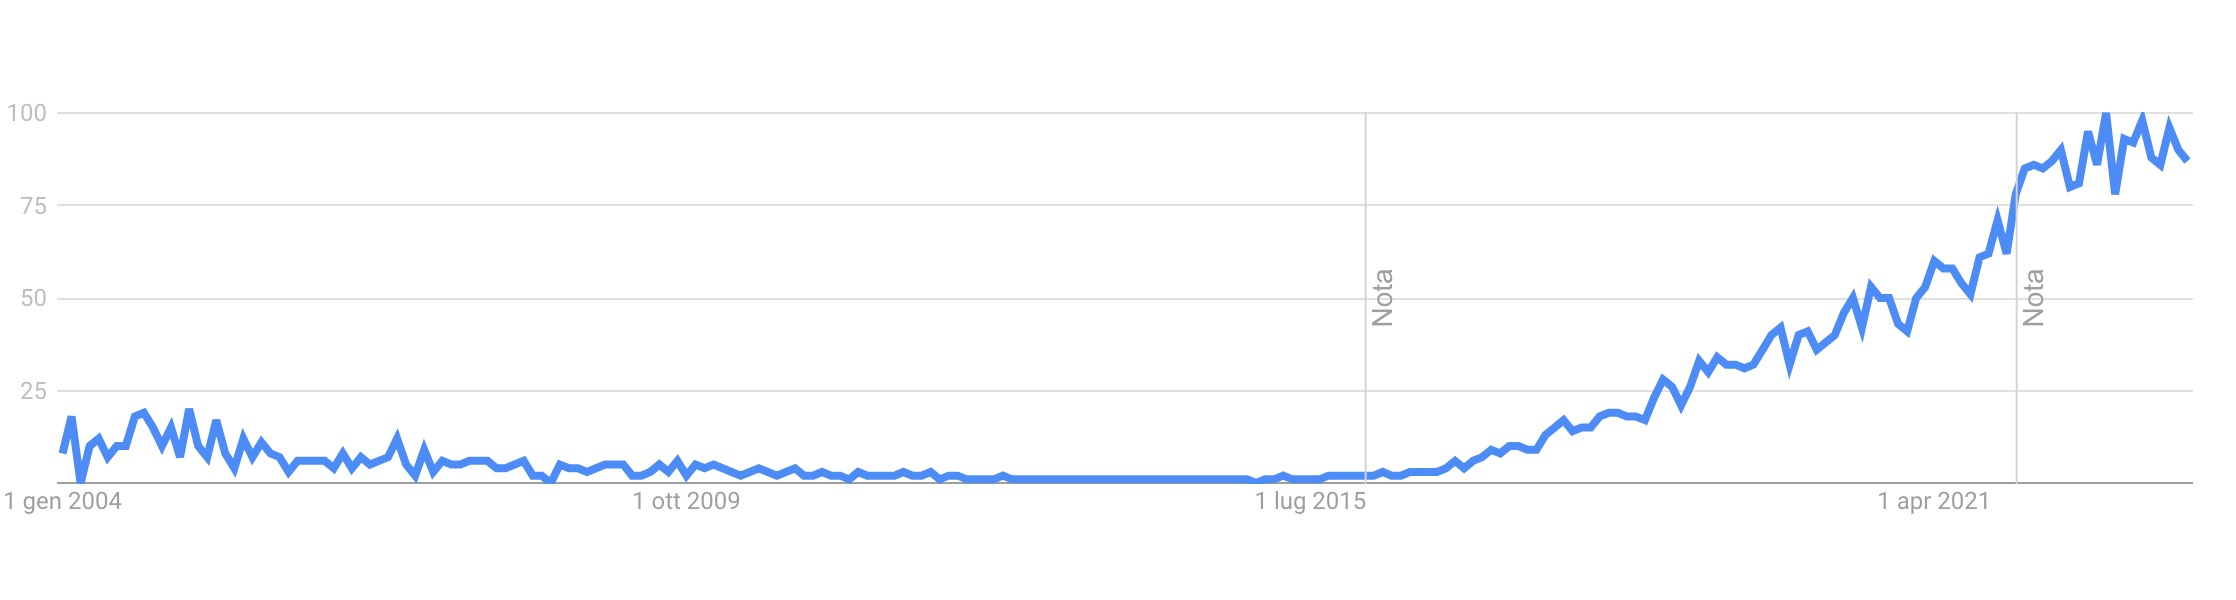
\includegraphics[width=12cm]{images/Trends_DT.jpg}
\caption[Grafico Google Trends ricerche sul Digital Twin]{Ricerche su \emph{Digital Twin} effettuate dal 2004 al 2023 su Google~\cite{Trends_DT}}\label{fig:trends}
\end{center}
\end{figure}

\subsection{Introduzione del Digital Twin}
Con l'avvento dell'Industria 4.0 il \emph{Digital Twin} è considerato di estrema importanza. I vari utilizzi del \emph{Digital Twin} in diversi settori includono la progettazione, pianificazione, ottimizzazione, manutenzione, sicurezza, presa di decisioni, accesso remoto e formazione. Può essere uno strumento prezioso per le aziende per aumentare la loro competitività, produttività ed efficienza~\cite{Campi_DT}.

\newpage

Il mercato globale del \emph{Digital Twin} è stato stimato a 3,1 miliardi di dollari nel 2020 e ci si aspetta che crescerà in modo esponenziale negli anni successivi (stimato intorno ai 137 miliardi per il 2030, figura \ref{fig:valutazione}).

\begin{figure}[h]
\begin{center}
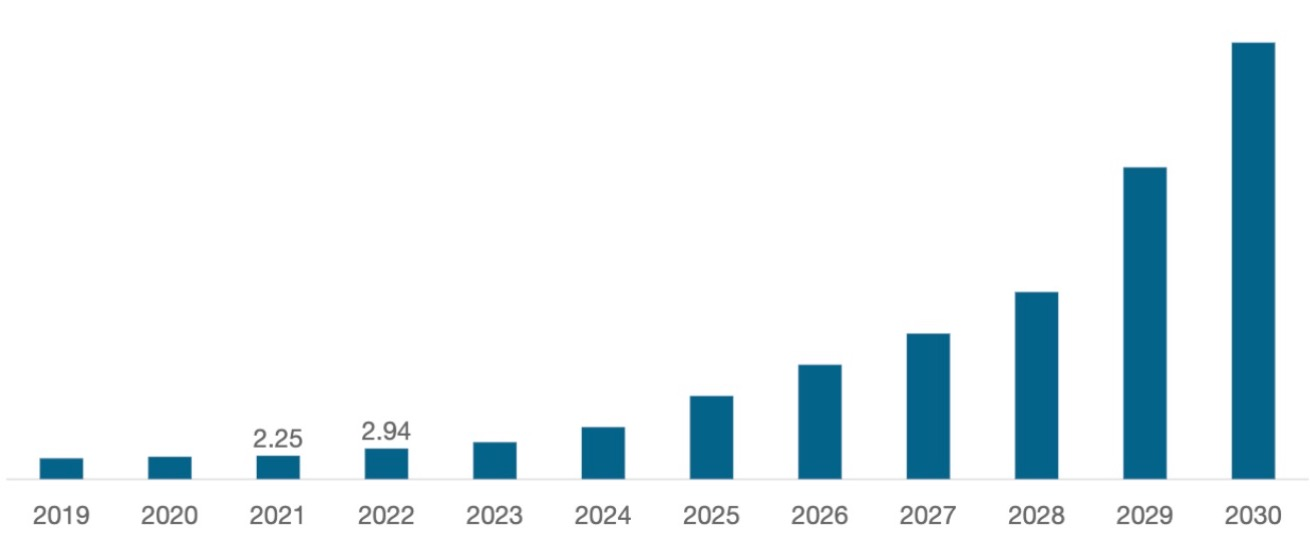
\includegraphics[width=12cm]{images/Market_DT.jpg}
\caption[Grafico valutazione Digital Twin]{Valutazione futura stimata sul \emph{Digital Twin}~\cite{Market_DT}}\label{fig:valutazione}
\end{center}
\end{figure}

La pandemia di COVID-19 ha cambiato il modo in cui vengono considerate la produzione e la manutenzione, accelerando l'adozione dei Digital Twin~\cite{Covid_DT}.

\subsection{Storia del Digital Twin}
Nonostante il \emph{Digital Twin} abbia guadagnato una grande popolarità negli ultimi anni, il concetto non è del tutto nuovo. Il suo concetto è emerso in relazione alla ”Gestione del Ciclo di Vita del Prodotto” nel 2002 presso l'Università del Michigan da Michael Grieves~\cite{Origin_DT}.

Il modello proposto ha tre componenti: prodotto reale, prodotto virtuale e un meccanismo di collegamento per il flusso di dati tra i due; il modello è stato poi chiamato ”Modello di Prodotti Specchiati”~\cite{Spazi_specchiati}. 

Un concetto simile, in cui i modelli software imitano la realtà a partire da informazioni provenienti dal mondo fisico, è stato immaginato da David Gelernter nel 1991 ed è stato chiamato ”Mondi Specchiati”~\cite{Mondi_specchiati}.

Entro il 2006, il nome del modello concettuale proposto da Grieves è stato cambiato da ”Modello di Prodotti Specchiati” a ”Modello di Riflessione delle Informazioni”~\cite{Origin_concept_DT, PLM_DT}.

Il nome \emph{Digital Twin} appare per la prima volta sotto forma di bozza in un articolo della NASA nel 2010~\cite{NASA2}. Nell'articolo della NASA, il \emph{Digital Twin} veniva anche definito ”Leader di Flotta Virtuale Digitale”. La NASA è stata la prima associazione a definire il \emph{Digital Twin}; è stato descritto come ”una simulazione integrata multi-fisica, multi-scala e probabilistica di un veicolo o sistema che utilizza i migliori modelli fisici disponibili, aggiornamenti dei sensori, storia della flotta, ecc., per riflettere la vita del suo gemello volante”~\cite{NASA}.

Anche se la prima menzione del \emph{Digital Twin} è nella roadmap del 2010, la NASA aveva utilizzato un concetto simile in passato per il programma Apollo, in cui venivano costruiti due veicoli spaziali identici per riflettersi a vicenda~\cite{Apollo}.

Successivamente la ”U.S. Air Force” ha seguito le orme della NASA ed ha utilizzato il \emph{Digital Twin} per la progettazione, la manutenzione e la previsione dei loro aerei~\cite{Air_force}. L'idea era quella di utilizzare il \emph{Digital Twin} per simulare le proprietà fisiche e meccaniche dell'aeromobile per prevedere qualsiasi affaticamento o crepa nella struttura.

Oltre al monitoraggio, il \emph{Digital Twin} è stato anche proposto per l'esplorazione spaziale sostenibile e per le future generazioni di veicoli aerospaziali~\cite{NASA}.

Dalla prima definizione mai pubblicata dalla NASA, diversi autori hanno descritto il \emph{Digital Twin} con termini propri e in base alla sua applicazione, definendolo come un modello virtuale~\cite{Fedelta, Airframe_DT, Def_DT, Def2_DT, Gerarchico, Complex_Aerostructures, DTH_DT}, una controparte digitale~\cite{Controparte1, Evolutivo}, un doppione ~\cite{IBM_DT}, un clone~\cite{Clone_DT} o una rappresentazione digitale~\cite{Rappresentazione1, Rappresentazione2, Rappresentazione3}.

Dopo che il \emph{Digital Twin} ha trovato un utilizzo in settori oltre la produzione, si è iniziato ad applicarlo anche ad entità biologiche complesse come gli esseri umani e gli alberi~\cite{Rappresentazione1, Alberi_DT}.

\newpage

Il \emph{Digital Twin} può svolgere compiti come:
\begin{itemize}
    \item Analisi approfondita del gemello fisico
    \item Progettazione e convalida di prodotti/processi nuovi o esistenti
    \item Simulazione delle condizioni di salute del gemello fisico
    \item Miglioramento della sicurezza e dell'affidabilità del gemello fisico
    \item Ottimizzazione di parti, prodotti, processi o linee di produzione
    \item Monitoraggio dello stato del gemello fisico durante tutta la sua vita
    \item Previsione delle prestazioni del gemello fisico
\end{itemize}

Le definizioni di \emph{Digital Twin} spesso trascurano la sua longevità; tuttavia, alcuni articoli considerano il \emph{Digital Twin} come un modello ”cradle-to-gravel ” (tradotto in italiano come ”dalla culla alla tomba”), significando che può essere utilizzato per l'intero ciclo di vita del prodotto, dal momento dell'ideazione fino alla sua eliminazione~\cite{Airframe_DT, Air_force, Culla, Culla2}.

Alcuni articoli~\cite{Economico} suggeriscono anche che il \emph{Digital Twin} può includere informazioni relative allo smaltimento del prodotto durante la fase di eliminazione. Inoltre, dopo che il prodotto è stato eliminato, il \emph{Digital Twin} può aiutare nella progettazione e produzione della generazione successiva~\cite{Riutilizzo}.

Il \emph{Digital Twin} è diverso dai modelli informatici (CAD/CAE) e dalla simulazione. Anche se molte organizzazioni lo utilizzano sinonimo a modello 3D, un modello 3D è solo una parte del \emph{Digital Twin}~\cite{Culla}.

Il \emph{Digital Twin} utilizza dati per riflettere il mondo reale in qualsiasi momento e quindi può essere utilizzato per osservare e comprendere le prestazioni del sistema e per la sua manutenzione predittiva~\cite{Sofisticazione}.

\newpage

\subsection{Vantaggi e caratteristiche del Digital Twin}
Dal momento in cui è stato introdotto per la prima volta, il \emph{Digital Twin} ha guadagnato sempre più popolarità, con sempre più ricercatori che hanno iniziato a concentrare la propria ricerca su questo argomento (figura \ref{fig:crescita_pubblicazioni}).

\begin{figure}[h]
\begin{center}
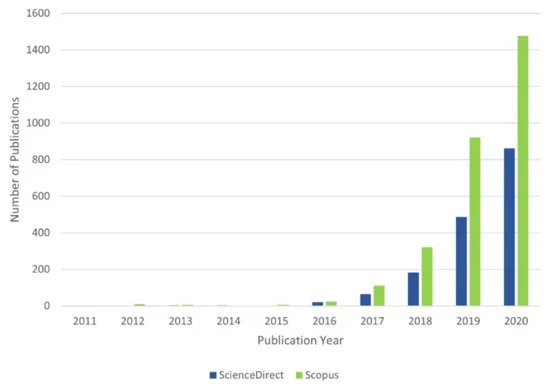
\includegraphics[width=12cm]{images/Pubblicazione_DT.jpg}
\caption[Grafico pubblicazione Digital Twin]{Trend di crescita sulla pubblicazioni del \emph{Digital Twin}~\cite{Researchgate}}\label{fig:crescita_pubblicazioni}
\end{center}
\end{figure}

La crescente popolarità del \emph{Digital Twin} è evidente dal fatto che è stato considerato come un argomento di tendenza nel campo tecnologico per tre anni consecutivi (2017-2019) da Gartner\cite{Gartner2017, Gartner2018, Gartner2019}, una tecnologia futura nel campo aerospaziale e della difesa da Lockheed Martin~\cite{Martin} e una delle tecnologie definitorie del prossimo decennio da Forbes~\cite{Forbes}

\newpage

\subsubsection{Vantaggi del Digital Twin}

La principale ragione per cui la tecnologia \emph{Digital Twin} è vista come la pietra angolare dell'Industria 4.0 risiede nella sua serie di vantaggi, che includono la riduzione di errori, incertezze, inefficienze e spese in qualsiasi sistema o processo. Inoltre, elimina tutti i compartimenti stagni nei processi o nelle organizzazioni che altrimenti operano in isolamento nelle strutture industriali più tradizionali. Alcuni dei vantaggi riportati per il \emph{Digital Twin} includono:
\begin{itemize}
    \item Velocità nella creazione e testing di un prototipo
    
    Poiché le simulazioni consentono l'analisi di numerosi scenari, i cicli di progettazione e analisi si accorciano, rendendo l'intero processo di lavoro con i prototipi più facile e veloce. Una volta implementato, il \emph{Digital Twin} può essere utilizzato in diverse fasi del processo di progettazione del prodotto, dalla concezione dell'idea del prodotto ai test~\cite{Testing_prototipo}. Poiché il \emph{Digital Twin} è collegato al suo gemello fisico per tutta la sua durata di testing, è possibile confrontare le prestazioni effettive e previste~\cite{Testing}.
    
    \item Economico
    
    Grazie al fatto che il \emph{Digital Twin} coinvolge principalmente risorse virtuali per la sua creazione, il costo complessivo di prototipazione diminuisce nel tempo.
    Nella prototipazione tradizionale, il ridisegno di un prodotto è dispendioso in termini di tempo e costi a causa dell'uso di materiali fisici e manodopera. Inoltre, un test che fallisce significa la fine di quel costoso prototipo. Utilizzando il \emph{Digital Twin}, i prodotti possono essere ricreati e sottoposti a test con alta probabilità di fallimento senza alcun costo aggiuntivo per i materiali. Quindi, assumendo che il costo sia uguale all'inizio, i costi fisici aumentano man mano che l'inflazione sale, ma i costi virtuali diminuiscono significativamente nel tempo~\cite{Economico}. Il \emph{Digital Twin} consente il testing dei prodotti in diverse situazioni operative, comprese quelle distruttive, senza costi aggiuntivi. Inoltre può ridurre i costi operativi e prolungare la vita utile delle attrezzature e degli asset una volta implementato.
    
    \item Previsione dei problemi
    
    Utilizzando il \emph{Digital Twin}, possiamo prevedere i problemi e gli errori per gli stati futuri del prodotto effettivo. Grazie ai dati in tempo reale che fluiscono tra l'oggetto fisico e il suo gemello digitale è possibile prevedere problemi durante le diverse fasi del ciclo di vita del prodotto. Questo è particolarmente vantaggioso per la gestione di strutture complesse che sono composte da materiali multipli come aerei, veicoli, attrezzature di fabbrica, ecc., poiché all'aumentare della complessità di un prodotto, diventa più difficile prevedere i guasti dei componenti con metodi convenzionali~\cite{Testing_prototipo}.
    
    \item Accessibilità
    
    Il dispositivo fisico può essere controllato e monitorato a distanza utilizzando il suo \emph{Digital Twin}. A differenza dei sistemi fisici, che sono limitati dalla loro posizione geografica, i sistemi virtuali (come il \emph{Digital Twin}) possono essere ampiamente condivisi e accessibili da remoto~\cite{Economico}. Il monitoraggio e il controllo a distanza di apparecchiature e sistemi diventano necessari in situazioni in cui l'accesso locale è limitato, come durante la pandemia di COVID-19 quando i governi hanno imposto blocchi e il lavoro a distanza o il contatto zero sono l'unica opzione praticabile~\cite{Covid_DT}.
    
    \item Sicurezza
    
    In settori come il settore petrolifero o minerario dove le condizioni di lavoro sono estremamente pericolose, la capacità del \emph{Digital Twin} di accedere da remoto al suo gemello fisico, così come la sua natura predittiva, può ridurre il rischio di incidenti e guasti pericolosi. Tuttavia, il vantaggio del \emph{Digital Twin} nell'accesso remoto non si limita alla prevenzione degli incidenti. Secondo un sondaggio di Gartner, quasi un terzo delle aziende ha utilizzato il \emph{Digital Twin} durante la pandemia per aumentare la sicurezza dei dipendenti e dei clienti attraverso il monitoraggio a distanza~\cite{Gartner_covid}.
    
    \item  Riduzione dei rifiuti

    Utilizzare il \emph{Digital Twin} per simulare e testare prototipi di prodotti in un ambiente virtuale riduce significativamente lo spreco di materiali. I prototipi possono essere sondati e controllati virtualmente, sotto una varietà di scenari di test diversi, per finalizzare il design del prodotto finale prima della produzione. Ciò non solo risparmia lo spreco di materiali, ma riduce anche i costi di sviluppo e il tempo di commercializzazione.

    \item Formazione del personale
    
    Il \emph{Digital Twin} può essere utilizzato per sviluppare programmi di formazione sulla sicurezza più efficienti e illustrativi rispetto a quelli tradizionali~\cite{Formazione}. Prima di operare in un ambiente ad alto rischio o su macchinari pericolosi, è possibile fornire agli operatori un addestramento attraverso l'utilizzo di un  \emph{Digital Twin} al fine di mitigare i rischi. L'istruzione relativa a vari processi o scenari li preparerà adeguatamente affinché possano affrontare in sicurezza situazioni simili di persona. Ad esempio, l'ambiente minerario è un ambiente ad alto rischio in cui i nuovi dipendenti possono essere addestrati utilizzando il \emph{Digital Twin} sull'utilizzo dei macchinari e su come affrontare scenari di emergenza~\cite{Mining}.
    
\end{itemize}

\newpage

\subsubsection{Caratteristiche del Digital Twin}

A seconda del tipo di \emph{Digital Twin}, può possedere proprietà distintive da altri, ma comunque tutti i \emph{Digital Twin} condividono alcune caratteristiche comuni:
\begin{itemize}
    \item Alta fedeltà
    
    Un \emph{Digital Twin} deve essere una copia quasi identica del suo gemello fisico in termini di aspetto, contenuti, funzionalità. Un modello digitale super realistico aiuta il \emph{Digital Twin} a imitare ogni aspetto del suo gemello fisico. I modelli informatici ad alta fedeltà sono considerati il suo fondamento. Questo livello di dettaglio consente agli strumenti di simulazione e previsione di essere più affidabili quando presentati con un insieme di azioni o scenari alternativi~\cite{Fedelta}.

    \item Dinamico

    Siccome il piano fisico è un sistema dinamico (a differenza del piano virtuale)  un \emph{Digital Twin} deve cambiare di conseguenza. Questo viene raggiunto attraverso la connessione continua e lo scambio di informazioni tra il mondo fisico e virtuale. Lo scambio di dati può riguardare dati dinamici, dati statici storici e dati statici descrittivi~\cite{Evolutivo}. L'obiettivo del \emph{Digital Twin} è di riflettere il comportamento del prodotto nel mondo digitale in qualunque momento~\cite{Culla}.

    \item Auto-evolutivo

    Il \emph{Digital Twin} si evolve insieme al suo gemello fisico durante l'intero ciclo di vita. Qualsiasi cambiamento sia nel \emph{Digital Twin} che nel prodotto è riflesso nell'altro, creando un ciclo di feedback continuo~\cite{Culla}. Un \emph{Digital Twin} è auto-adattante e auto-ottimizzante grazie ai dati raccolti dal gemello fisico in tempo reale, maturando quindi insieme al suo gemello fisico durante tutta la sua durata~\cite{Evolutivo}.

    \newpage

    \item Identificabile
    
    Ogni componente deve avere il proprio \emph{Digital Twin}. Durante diverse fasi del ciclo di vita del prodotto, i dati e le informazioni ad esso correlati si evolvono (inclusi modelli geometrici 3D, modelli di produzione, modelli di utilizzo, modelli funzionali, ecc ...). Grazie all'esistenza di tali modelli creati per il \emph{Digital Twin}, esso può essere identificato univocamente dal suo gemello fisico o viceversa per l'intera durata del suo ciclo di vita~\cite{Identificabile}.
    
    \item Gerarchico
    
    La natura gerarchica del \emph{Digital Twin} deriva dal fatto che i diversi componenti e parti che compongono il prodotto finale hanno il proprio modello \emph{Digital Twin} corrispondente, ad esempio il \emph{Digital Twin} di un aereo è composto da \emph{Digital Twin} di una specifica componente, \emph{Digital Twin} del sistema di controllo di volo, \emph{Digital Twin} del sistema di propulsione, ecc. Pertanto, un \emph{Digital Twin} può essere visto come una serie di sub-modelli integrati~\cite{Gerarchico}.
    
\end{itemize}

\subsection{Categorie del Digital Twin}
Il \emph{Digital Twin} può essere categorizzato in base alle sua applicazione~\cite{Economico}.

Le due principali applicazioni di un \emph{Digital Twin} sono la previsione e l'interrogazione~\cite{Economico}.
Un \emph{Digital Twin} predittivo, come suggerisce il nome, prevede il comportamento e le prestazioni future del suo corrispettivo fisico, mentre un \emph{Digital Twin} interrogativo è utilizzato per interrogare lo stato attuale o passato del suo corrispettivo fisico indipendentemente dalla sua posizione~\cite{Categoria}.

\newpage

I \emph{Digital Twin} possono anche essere suddivisi a seconda se l'attenzione dell'applicazione è sul prodotto, sul processo o sulle prestazioni~\cite{Categoria}:
\begin{itemize}
    \item \emph{Digital Twin} di Prodotto
    
    Viene utilizzato per la fase di gestione del prototipo poiché analizza il prodotto in diverse condizioni e si assicura che il successivo prodotto fisico si comporti come previsto. Questa fase può essere rapida in quanto il tempo di sviluppo complessivo viene ridotto e non è più necessario svilupparne molti.

    \item \emph{Digital Twin} di Produzione
    
    Viene utilizzato per convalidare i processi simulandoli e quindi analizzandoli anche prima della produzione effettiva. Ciò aiuta a sviluppare una metodologia di produzione efficiente in diverse condizioni. I dati provenienti dai \emph{Digital Twin} di Prodotto e Produzione possono essere utilizzati insieme per il monitoraggio e la manutenzione delle macchine.
    
    \item \emph{Digital Twin} di Prestazioni
    
    Viene utilizzato per i processi decisionali catturando, aggregando e analizzando i dati provenienti da prodotti e impianti intelligenti. Poiché il \emph{Digital Twin} di Prestazioni include le prestazioni sia del prodotto che della produzione, ottimizza le operazioni in base alla disponibilità delle risorse dell'impianto, creando un'opportunità per migliorare i \emph{Digital Twin} di Produzione e Prodotto attraverso un ciclo di feedback.
\end{itemize}

\newpage

\subsection{Gerarchia del Digital Twin}

Da una prospettiva gerarchica, i \emph{Digital Twin} possono essere suddivisi anche in tre diversi livelli (figura \ref{fig:gerarchia}), in base all'entità coinvolta nella produzione~\cite{Identificabile}:


\begin{figure}[h]
\begin{center}                      
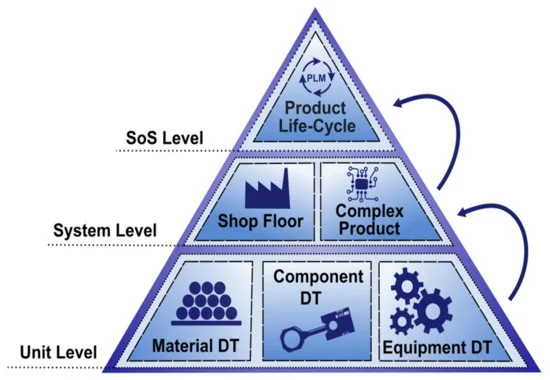
\includegraphics[width=10cm]{images/Gerarchia_DT.png}
\caption[Gerarchia del Digital Twin]{Gerarchia del Digital Twin}\label{fig:gerarchia}
\end{center}
\end{figure}

\begin{itemize}
    \item Livello di Unità (Unit level)
    
    È l'unità più piccola nella produzione e può essere un pezzo di attrezzatura, materiale o un fattore ambientale. Il \emph{Digital Twin} a livello di unità si basa sul modello geometrico, funzionale, comportamentale e operativo del corrispettivo fisico.

    \item Livello di Sistema (System level)
    
    È un'aggregazione di diversi \emph{Digital Twin} di livello unità in un sistema di produzione (come per esempio una fabbrica). L'interconnettività e la collaborazione tra molteplici \emph{Digital Twin} a livello di unità portano a un flusso più ampio di dati e a una migliore allocazione delle risorse. Un prodotto complesso, ad esempio un aereo, può essere considerato anche come \emph{Digital Twin} a livello di sistema.

    \item Livello di Sistema di Sistemi (SoS level)
    
    Un certo numero di \emph{Digital Twin} di livello di sistema è collegato insieme per formarne uno a livello di SoS, che aiuta la collaborazione tra diverse aziende o tra diversi dipartimenti di un'azienda (come la catena di approvvigionamento, il design, il servizio, la manutenzione). In altre parole, il \emph{Digital Twin} a livello di SoS integra diverse fasi del prodotto durante tutto il suo ciclo di vita.

\end{itemize}

\subsection{Livello di Maturità/Sofisticazione}

In base al livello di sofisticazione dei \emph{Digital Twin}, ovvero alla quantità e alla qualità dei dati ottenuti dal gemello fisico e dal suo ambiente, i \emph{Digital Twin} possono essere raggruppati in~\cite{DT_tipi}:

\begin{itemize}
    \item Digital Twin Parziale
    
    Contiene un piccolo numero di punti dati, ad esempio pressione, temperatura, umidità, ecc., utili per determinare la connettività e la funzionalità del \emph{Digital Twin}.

    \item Digital Twin Clone
    
    Contiene tutti i dati significativi e rilevanti provenienti dal prodotto/sistema che possono essere utilizzati per la creazione di prototipi e la categorizzazione delle fasi di sviluppo.

    \item Digital Twin Potenziato
    
    Utilizza i dati del gemello fisico insieme ai suoi dati storici e elabora i dati utili utilizzando algoritmi e analisi.
\end{itemize}

\newpage

I \emph{Digital Twin} possono diventare più sofisticati e precisi con l'accumulo di insiemi di dati più ampi nel corso del tempo di funzionamento. Il livello di maturità dei \emph{Digital Twin} non è limitato solo ai dati, ma comprende anche il livello di sofisticazione della rappresentazione/modello virtuale. Su questa base, i \emph{Digital Twin} sono suddivisi in quattro livelli~\cite{Sofisticazione}:

\begin{enumerate}
    \item Pre-Digital Twin
    
    Questo è il livello 1, in cui il \emph{Digital Twin} viene creato prima dell'asset fisico con lo scopo di prendere decisioni sul design del prototipo per ridurre qualsiasi rischio tecnico e risolvere anticipatamente i problemi utilizzando un modello di sistema generico.

    \item Digital Twin
    
    Il livello 2 incorpora i dati dell'asset fisico relativi alle sue prestazioni, salute e manutenzione. Il modello virtuale del sistema utilizza questi dati per assistere le decisioni ad alto livello nella progettazione e nello sviluppo dell'asset, insieme alla pianificazione della manutenzione. Il trasferimento dei dati a questo livello è bidirezionale.

    \item Digital Twin Adattativo
    
    Il livello 3 fornisce un'interfaccia utente adattiva tra l'asset fisico e il \emph{Digital Twin} e ha la capacità di imparare dalle preferenze e dalle priorità degli operatori umani utilizzando il machine learning supervisionato. Utilizzando questo \emph{Digital Twin}, è possibile la pianificazione e la presa di decisioni in tempo reale durante le operazioni.
    
    \item Digital Twin Intelligente
    
    Oltre alle caratteristiche del livello 3, il livello 4 ha la capacità di apprendimento automatico non supervisionato, rendendolo più autonomo rispetto al livello 3. Può riconoscere modelli nell'ambiente operativo e utilizzando questi dati insieme all'apprendimento rinforzato consente un'analisi più precisa ed efficiente del sistema.
    
\end{enumerate}

\section{Digital Thread}
Proprio come il concetto di \emph{Digital Twin}, il termine \emph{Digital Thread} nasce dall'industria aerospaziale, dove è nato come parte integrante di un processo di ingegneria dei sistemi avanzato, mirato alla gestione completa e digitale di tutte le fasi coinvolte. Inizialmente concepito per tracciare e coordinare le varie fasi di progettazione, produzione e distribuzione di un sistema complesso, il \emph{Digital Thread} si è rivelato fondamentale per la sincronizzazione di dati e informazioni lungo l'intero ciclo di vita del prodotto~\cite{Thread}.

Questo contesto pionieristico nell'industria aerospaziale ha visto il \emph{Digital Thread} come una rete intricata di molteplici dati, dai modelli CAD 3D alle strategie di produzione, dai dettagli logistici ai processi di assemblaggio~\cite{Thread2}.

Una delle sue caratteristiche principali è la capacità di fornire un flusso ininterrotto di informazioni, garantendole disponibili sempre disponibili a richiesta(figura \ref{fig:dth_example}). Rispetto al \emph{Digital Twin}, che funge da gemello virtuale in tempo reale di un oggetto fisico, il \emph{Digital Thread} agisce come una traccia storica, una sorta di cronologia digitale che registra e conserva ogni tappa e aspetto del ciclo di vita dell'oggetto fisico~\cite{Thread3}.

\begin{figure}[h]
\begin{center}
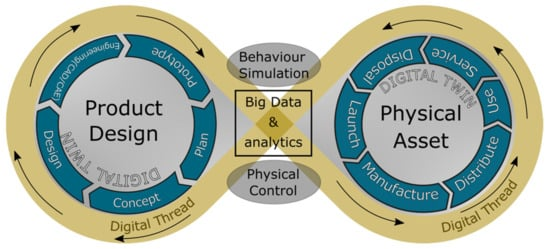
\includegraphics[width=12cm]{images/Example_DTH.jpg}
\caption[Esempio funzionamento Digital Thread]{Esempio funzionamento del \emph{Digital Thread}~\cite{Thread3}}\label{fig:dth_example}
\end{center}
\end{figure}

\newpage

Il \emph{Digital Thread} è uno dei fondamenti su cui si basa l'Industria 4.0. La convergenza di principi come l'\emph{Internet of Things} (IoT) – che consente ai dispositivi di raccogliere e scambiare dati –, la virtualizzazione, la decentralizzazione delle decisioni e la capacità di analizzare dati in tempo reale costituiscono esempi in cui viene altamente adottato l'intero concetto di \emph{Digital Thread}~\cite{Thread}.

\subsection{Vantaggi e Applicazioni}

L'implementazione del concetto del \emph{Digital Thread} ha dimostrato di portare molti benefici in diversi settori~\cite{Thread4}. La tracciabilità completa e digitale dei dati lungo l'intero ciclo di vita del prodotto ha un impatto significativo sull'efficienza operativa, sulla riduzione degli errori, sull'accelerazione dei tempi di produzione e sulla possibilità di offrire personalizzazione su larga scala~\cite{Thread}.

\begin{itemize}
    \item Miglioramento dell'Efficienza Operativa

    La capacità di tracciare ogni fase di un prodotto attraverso il \emph{Digital Thread} consente un controllo più rigoroso e una gestione ottimizzata dei processi. Ciò si traduce in una maggiore efficienza nella pianificazione e nell'esecuzione delle attività di produzione. Ad esempio, le aziende manifatturiere possono monitorare in tempo reale l'utilizzo delle risorse, identificando aree di sovrautilizzo o sottoutilizzo e apportando correzioni tempestive.

    \item Riduzione degli errori
    
    L'automazione del flusso di dati all'interno del \emph{Digital Thread} riduce significativamente il rischio di errori umani. Gli errori di trascrizione e di comunicazione vengono minimizzati poiché le informazioni vengono trasferite e condivise in modo accurato e coerente tra le diverse fasi del processo produttivo. Questo aspetto è particolarmente rilevante in settori ad alta precisione, come l'industria medica, dove anche un piccolo errore potrebbe avere conseguenze significative.

    \item Accelerazione dei tempi di produzione

    La collaborazione e l'accesso in tempo reale alle informazioni attraverso il \emph{Digital Thread} consentono una pianificazione più agile e una riduzione dei tempi di attesa. La condivisione istantanea di dati tra diversi reparti, fornitori e partner durante la produzione accelera il processo decisionale e riduce i ritardi.

    \item Personalizzazione su larga scala

    Uno dei vantaggi distintivi del \emph{Digital Thread} è la sua capacità di consentire la personalizzazione su larga scala. La tracciabilità digitale delle specifiche del prodotto e delle preferenze dei clienti consente la progettazione e la produzione di prodotti altamente personalizzati, senza sacrificare l'efficienza. Ad esempio, nell'industria dell'abbigliamento, le aziende possono creare capi su misura basati sui dati delle misurazioni dei clienti.
    
    \item Applicazioni in diversi settori
    
    Oltre all'industria aerospaziale, il concetto di \emph{Digital Thread} ha trovato applicazione in diverse altre industrie. Nel settore energetico, la gestione digitale delle risorse permette un monitoraggio continuo delle prestazioni e una manutenzione preventiva più efficace. Nell'industria alimentare, il \emph{Digital Thread} può tracciare l'intera filiera di produzione, aumentando la trasparenza e la sicurezza alimentare. Anche l'industria farmaceutica beneficia della tracciabilità digitale per garantire la conformità normativa e la sicurezza dei prodotti~\cite{Thread5}.
    
\end{itemize}

\newpage

\section{Digital shadow}

Nell'era contemporanea, il termine \emph{Digital Shadow} è emerso come un concetto che riflette l'impatto delle attività online sulla creazione di una sorta di ”ombra digitale”. Questo fenomeno rappresenta il riflesso virtuale delle azioni, delle interazioni e delle informazioni che lasciamo dietro di noi mentre interagiamo con il mondo digitale~\cite{Shadow}.

\subsection{Definizione}

Il \emph{Digital Shadow} rappresenta il complesso aggregato di dati, tracce digitali e informazioni personali che lasciamo involontariamente o volontariamente durante le nostre attività online. Questo spazia dalle ricerche su motori di ricerca, alle interazioni sui social media, agli acquisti online, alle conversazioni tramite e-mail e molto altro ancora. In altre parole, è la traccia virtuale che si forma attraverso le azioni nell'ambiente digitale. Questi dati vengono quindi utilizzati per profilare gli utenti, personalizzare le esperienze digitali e, in alcuni casi, per fini pubblicitari e di marketing~\cite{Shadow}.

\subsection{Vantaggi del \emph{Digital Shadow}}

Il \emph{Digital Shadow} ha portato a molteplici sviluppi positivi nella società moderna~\cite{Shadow}:

\begin{itemize}
    \item Personalizzazione delle esperienze
    
    Grazie al \emph{Digital Shadow}, le piattaforme possono offrire contenuti e servizi personalizzati, adattati alle preferenze individuali, migliorando così l'esperienza dell'utente.

    \item Avanzamenti tecnologici
    
    L'analisi dei dati del \emph{Digital Shadow} ha contribuito alla creazione di algoritmi di intelligenza artificiale e di apprendimento automatico, che guidano l'innovazione in vari settori, come la medicina, l'automazione industriale e altro ancora.

    \item Ricerca e innovazione
    
    Gli scienziati e i ricercatori possono utilizzare dati anonimi del \emph{Digital Shadow} per ottenere informazioni preziose sui modelli di comportamento e sulle tendenze sociali, facilitando così la ricerca e l'innovazione~\cite{Shadow2}.
\end{itemize}

\subsection{Preoccupazioni del \emph{Digital Shadow}}

Tuttavia, il concetto di \emph{Digital Shadow} suscita anche preoccupazioni significative, tra cui:

\begin{itemize}
    \item Privacy
    
    La raccolta e l'archiviazione dei dati del \emph{Digital Shadow} sollevano interrogativi sulla privacy individuale. La condivisione non autorizzata di informazioni personali può portare a violazioni della privacy e all'abuso delle informazioni sensibili.
    
    \item Rischio di utilizzo malevolo
    
    I dati del \emph{Digital Shadow} possono essere vulnerabili agli attacchi informatici e all'uso malevolo da parte di attori maligni, mettendo a rischio la sicurezza delle informazioni personali.
\end{itemize}

\subsection{Economia dei dati}

L'accumulo di dati nel \emph{Digital Shadow} ha innescato una rivoluzione nell'economia dei dati, trasformando radicalmente la dinamica aziendale e le strategie di mercato. Aziende di tutte le dimensioni stanno riconoscendo il valore inestimabile dei dati e il potenziale che essi offrono per comprendere meglio i consumatori e anticipare le tendenze di mercato~\cite{Shadow, Shadow_economy}.

Questo nuovo paradigma ha visto la nascita di un'industria incentrata sulla raccolta, l'elaborazione e lo sfruttamento dei dati del \emph{Digital Shadow}. Le aziende investono ingenti risorse per sviluppare algoritmi sofisticati e sistemi di analisi dei dati che possono estrapolare conoscenze preziose dai comportamenti e dalle preferenze degli utenti. Questi dati sono poi venduti a inserzionisti, aziende di marketing e altre organizzazioni che cercano di perfezionare le proprie strategie di promozione.

In questo contesto, i dati sono diventati una vera e propria moneta di scambio. Le aziende possono acquisire vantaggi competitivi attraverso l'accesso a dati accurati e approfonditi sulle abitudini dei consumatori. Tuttavia, questa crescente dipendenza dai dati ha sollevato interrogativi sulla trasparenza e sulla giustizia dell'acquisizione e della monetizzazione di tali informazioni~\cite{Shadow_economy, Sell_data}.

\subsection{Etica e regolamentazione del \emph{Digital Shadow}}

L'espansione incontrollata del \emph{Digital Shadow} ha innescato una serie di sfide etiche e legali che richiedono una risposta ponderata e regolamentazioni adeguate. La rapida raccolta e condivisione di dati sensibili ha sollevato interrogativi fondamentali sulla privacy individuale e sulla sovranità dei dati personali~\cite{Shadow_economy, Sell_data, Sell_data2}.

L'equilibrio tra l'innovazione tecnologica e la protezione della privacy è al centro del dibattito pubblico e politico~\cite{Sell_data2, Sell_data}. I governi stanno lavorando per introdurre normative che regolamentino la raccolta e l'uso dei dati personali, garantendo il consenso informato degli individui e stabilendo sanzioni per violazioni ed abusi~\cite{Law_Data}. Tuttavia, trovare il giusto equilibrio tra il potenziale beneficio dell'analisi dei dati e la salvaguardia della privacy è un compito complesso.